\chapter{Results}

%Give a paragragh summary this chapter
This chapter will cover the result of experimenting OpenMP parallel directives to selected loops in order to observe possible speedup/slowdown through parallelization, hence give a conclusion and future work regarding RegCM potential improvement using GPU parallelization.Test Setup section explains how the test was conducted, including hardware used, dataset, testing parameter. Then, the result will be shown in the following section along with some comments regarding it. \\

\section{Test Setup}

The experiment had RegCM ran on different sets of hardware, both on serial mode (non MPI) and OpenMP parallel mode, then performance time was recorded for comparison. RegCM is a model simulation, so a large enough data set is needed. Fortunately, in the User Manual of RegCM, the development team has provided links to a handful of data set, containing climate models of a full year, from 1990 to the present. This test, however, will only use data set from 1990 and will let RegCM run simulations on this particular data set on different duration, from 1 month to 12 months. \\
~\\
There are two sets of hardware that was used on this experiment. The first workstation, named ICT4, has a 6-core, hyperthreaded Intel Xeon E-2620 v3, running at a clockspeed of 2.4 GHz, and can be boosted to 3.2 GHz. ICT4 also contains 32 GB of RAM. The second workstation, the ICT5, however, has 2 of the Intel Xeon E-2620 v3, making it a 12-core computer, with RAM capacity at 128GB. \\
~\\
The set of hardware in focus here is the ICT4. Comparison will be made between running RegCM on serial mode, 6 paralleled logical cores and 10 paralleled logical cores. Also, result of ICT4's 10 paralleled processors will also go up against that of the ICT5. One thing to note that, comparing serial computing performance between ICT4 and ICT5 is redudant. Basically, they have same the processing power in single-core performance as both have identical CPU. \\

\section{Results and Discussion}

First of all, Figure 4.1 below illustrates comparison between serialize and parallelize RegCM, perfomance-wise, on the ICT4. \\
\begin{figure}[H]
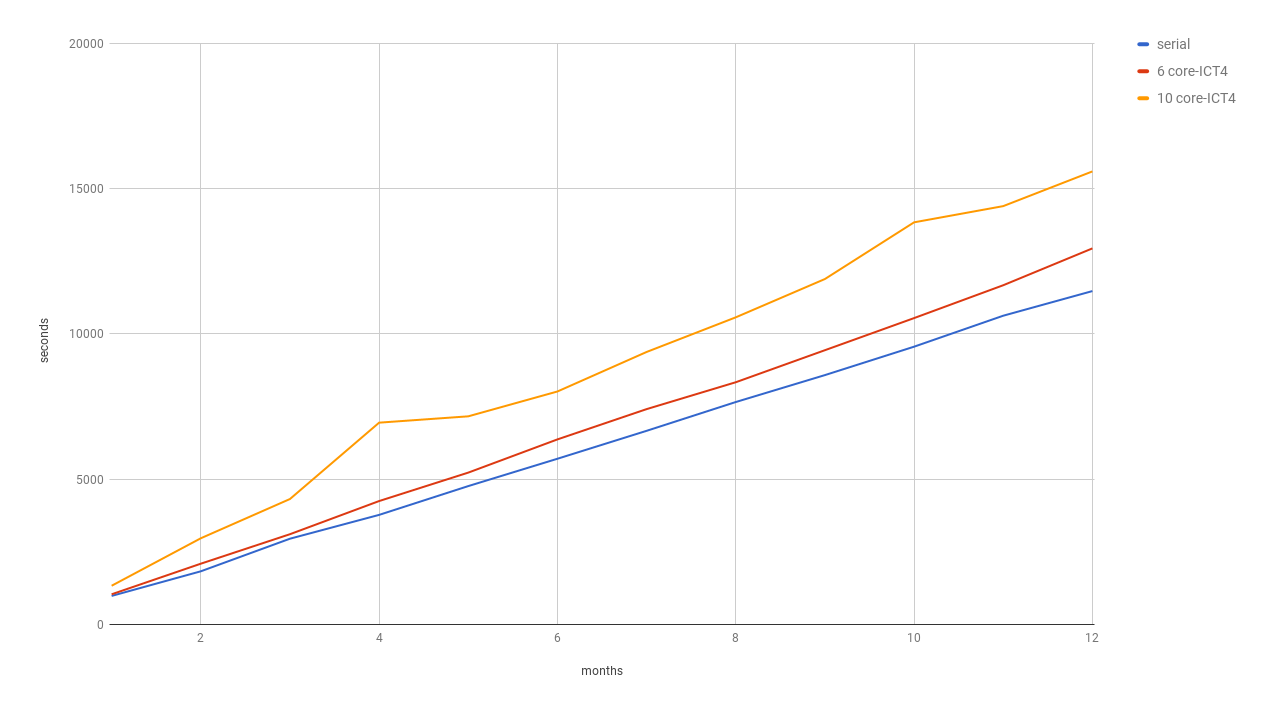
\includegraphics[width=11cm]{chart_ict4.png}
\centering
\caption{Parallel versus Serial Performance on ICT4}
\end{figure}
~\\
As can be seen, parallelized versions of RegCM using OpenMP on selected heavy computing for-loops actually performed worse than the serialize version. Possible explaination for this outcome can be one of the following: Either the for-loops that were parallelized with OpenMP contain data dependencies, which was mentioned in the previous chapter, or the number of loop iterations and the complexity of the computations are not great enough to benefit from parallelization, thus not out-weighting the extra overhead produced by task scheduling. The latter was demonstated more clearly the performance of 10-core parallel RegCM is put side by side with that of 6-core parallel version. The execution time is much more worse, which was caused by the time it takes to manifest, divide and schedule the work for 4 more logical cores. \\
~\\
After having ran OpenMP version of RegCM on both the ICT4 and ICT5, using the same number of processors, the result is shown in Figure 4.2
\begin{figure}[H]
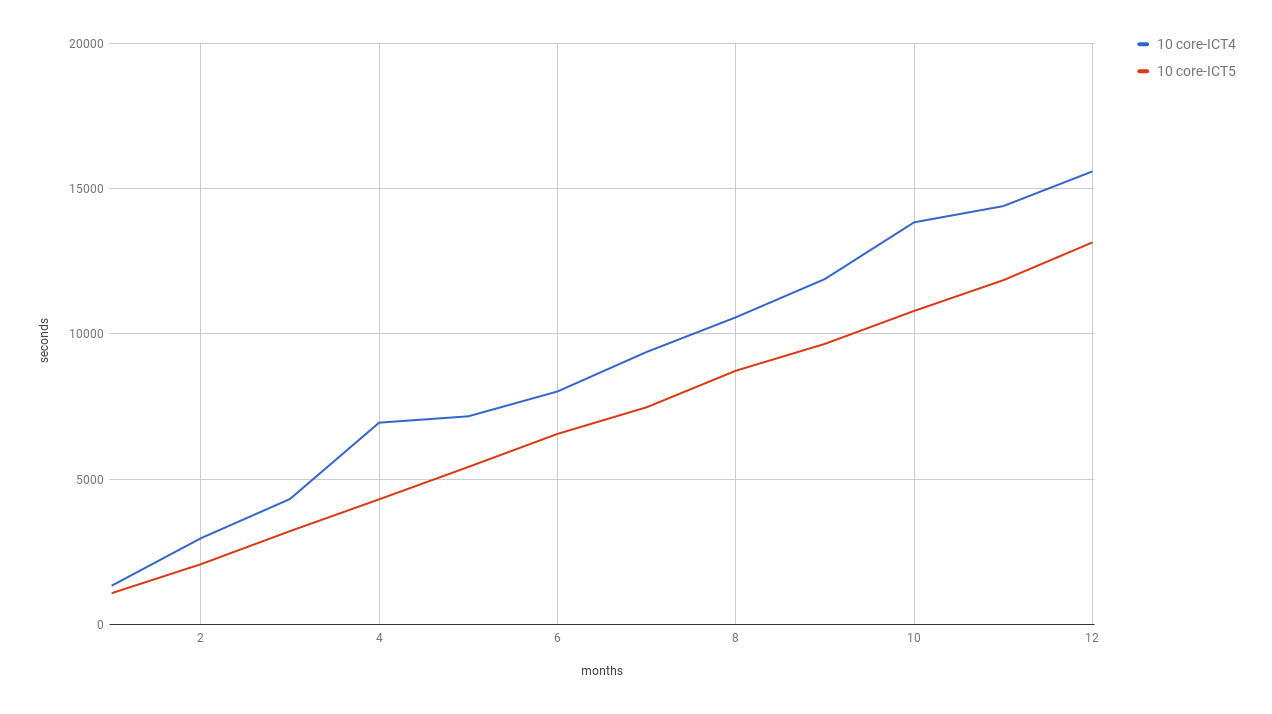
\includegraphics[width=11cm]{chart_ict5.png}
\centering
\caption{ICT4 versus ICT5 on 10-core performance}
\end{figure}
~\\
While having the same CPU model, the configuration of ICT4 and ICT5 affects the result greatly. Unlike the ICT4 which ran the simulation on 10 hyperthreaded core, the ICT5, with its multi CPUs configuration, ran RegCM with 10 physical core, thus reduced the overhead caused for task scheduling. Also execution time on ICT5 during the experiment shows more consistency. \\
~\\
A notable mention is that during earlier testing phase, there was a case where using OpenMP on RegCM displayed better performance than the original serialized program. However, how did that happen was unknown and it could not be re-created during the experiment.
